\chapter{引言}
\label{cha:intro}

\section{选题背景}

\subsection{云计算的历程}

云计算的概念诞生的远远比它的名字更早。它的概念可以追溯到早期的
分时系统\footnote{time-sharing systems}。

早期的计算机系统价格昂贵,而且体积庞大,使得个人用户很难拥有独立的个人计算机 (PC) 。
这就导致了多个用户可以同时使用同一个计算资源——例如一台电子计算机——的分时系统
~\cite{timesharing}的产生。所谓分时系统,就是有一个主要的
计算系统 (mainframe computer) ,用户通过终端机 (terminal) 连接到这个
系统上使用计算资源。用户一般而言不需要考虑计算机操作系统乃至硬件的具体细节——因为自然
有管理员管理这些细节,只需要像“租客”一样使用计算资源就可以了。现代的操作系统,
例如 GNU/Linux 或者 Microsoft Windows ,都支持多用户模式。

\begin{figure}[h]
    \centering
    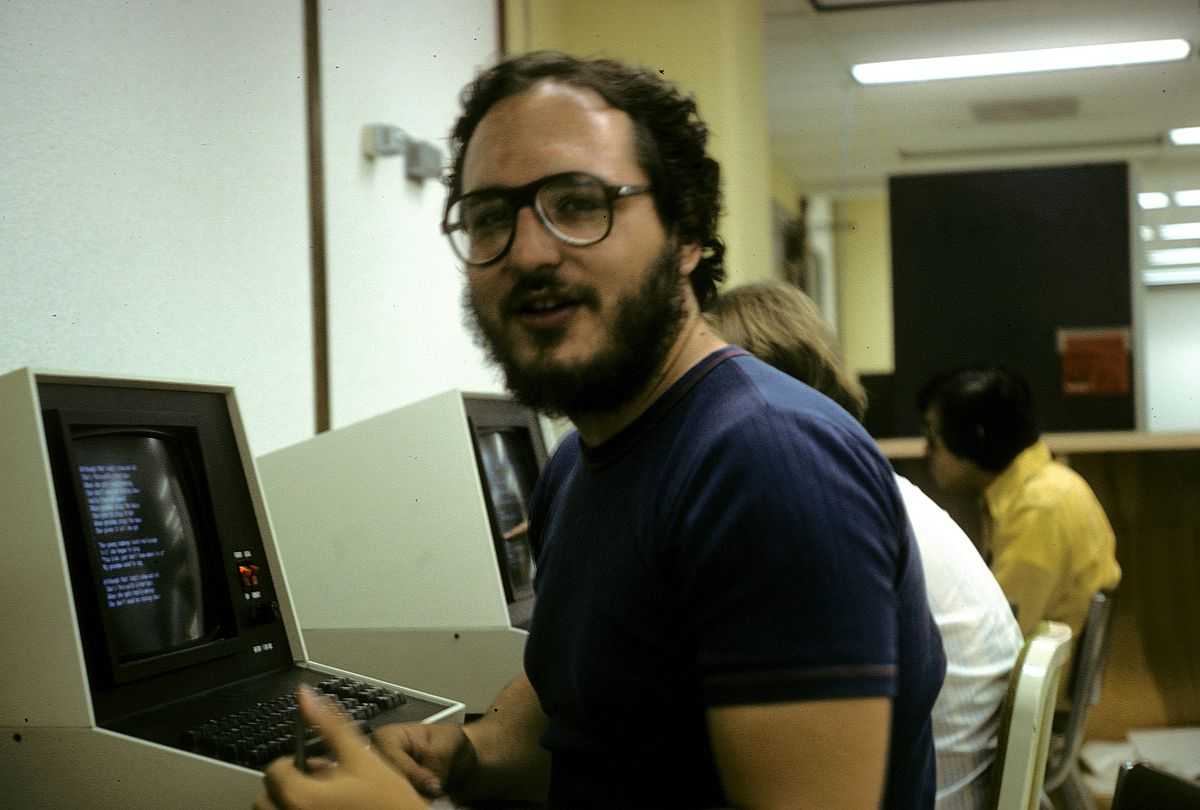
\includegraphics[height=0.5\textwidth]{unix_time_sharing}
    \caption{威斯康辛大学麦迪逊分校的学生使用终端机,1978 年}
\end{figure}

从 2000 年左右开始,云计算的概念正式形成了。2006 年诞生的 Amazon EC2 \footnote{EC2
  是 Elastic Compute Cloud 的缩写,因有两个连着的 C 所以叫做 EC2 ,不是
  “第二个版本”的意思。}成为了迄今最成功的云计算平台之一。2008 年诞生的 OpenNebula
是另一个云计算平台,顾名思义它是一个自由软件\footnote{Free as in freedom}
,使用 Apache License 发布。

而现在更加流行的自由的云计算平台是 OpenStack 。OpenStack 最初是由
 NASA 和 RackSpace 共同发起的,从 2012 年开始由叫做 OpenStack Foundation 的非营利
组织进行开发和维护。它和 Amazon EC2 的最大不同就是它是完全自由和开源的。不但可以利用
这个软件搭建自己的云计算环境,而且可以对相关的代码展开研究。OpenStack 中的主要组成部分
和 Amazon AWS 中的部分具有一定的对应关系,比如 AWS 的核心也就是 EC2 对应了 OpenStack
 里的 Nova ,负责虚拟机的调度和管理;AWS 中的简单存储模块 S3 在 OpenStack 中
有 Swift 与之对应~\cite{openstack}。

\subsection{云计算平台的服务类型}

云计算提倡的概念是“所有都是服务”
 (everything as a service) ~\cite{cloud-and-openstack},也就是用户不直接接触
物理上的计算机,但是却能通过网络获得相应的计算服务。云计算的“云”不在本地,这就好比大家
每天日常生活都要使用电,但极少有人在家里自己搭建一台柴油发电机,而是在发电厂集中发电,
然后通过输电线路把电力输送到千家万户供人们使用。数据中心就好像这个发电厂,计算机网络
就好像电线,终端用户就像使用电力一样使用云计算产生的计算资源。

根据服务类型不同,云计算平台主要可以分为以下三种——基础设施
服务 (IaaS)、平台服务 (PaaS) 还有软件服务 (SaaS) ~\cite{types-of-cloud}。

\subsubsection{基础设施服务}

顾名思义,这种服务类型就是只提供必要的设施,而不提供上层应用。这些设施包括由虚拟机管理程序
支持的大量的虚拟机集群、操作系统磁盘镜像存储池(这样用户在创建虚拟机实例的时候就不用联网
从镜像源下载镜像,直接从镜像存储服务调取相应的镜像即可)、文件存储服务、防火墙、负载均衡器
等等。

当然还有虚拟局域网。例如某大学计算机系有网络和操作系统两个实验室,它们共享一套虚拟机集群。
网络实验室和操作系统实验室希望各占用一个子网。如果是使用物理上的局域网,那么应该有两个交换机,
各接入路由器的两个物理端口上。而使用了虚拟局域网,就可以用两个逻辑端口代替。使用虚拟局域网,
可以缩小广播域,从而提高集群的安全性。

上文提到的 Amazon EC2 就是一个典型的 IaaS 平台。类似的,OpenStack 也是一个 IaaS 平台,
截至到 2016 年,一共包含以下几个核心组成部分:

\begin{enumerate}
    \item \textbf{Nova: }虚拟机管理
    \item \textbf{Neutron: }
    \item \textbf{Swift: }
    \item \textbf{Cinder: }
    \item \textbf{Keystone: }
    \item \textbf{Glance: }
\end{enumerate}


\subsubsection{平台服务}

\subsubsection{软件服务}

\subsection{虚拟化和云计算}

\section{研究价值和主要贡献}

\section{论文结构}
